\section{Mesures de performance et comparatifs}
	Dans la partie précédente, on s'est contenté de présenter différents tests de primalité sans conclure par rapport à leurs performances. Dans cette partie, on va mesurer ces performances et établir un comparatif entre les différents tests abordés.
	
	\subsection{Évolution des tests de primalité}
		Plusieurs algorithmes de tests de primalité se sont succédés au fil du temps. Des algorithmes de plus en plus efficaces apparaissent pour en remplacer d'autres.
	
		\subsubsection*{Premiers tests déterministes}
			\paragraph{}Les plus anciens algorithmes de tests de primalité sont les algorithmes de \textit{\textbf{test naïf}}, dont le \textit{\textbf{crible d'Erathostène}} qui date d'avant J-C. Ces algorithmes sont déterministes, c'est-à-dire qu'ils retournent toujours une réponse exacte. Ils constituent la façon la plus naturelle de tester la primalité d'un nombre mais leur complexité est trop élevée, surtout quand il s'agit de tester des grands nombres.
			
			\paragraph{}D'autres algorithmes déterministes basés sur des théorèmes plus récents sont aussi apparus, on peut citer le \textit{\textbf{test de Wilson}}. Il est énoncé pour la première fois par le mathématicien \textit{Ibn al-Haytham} dans les années 1000, puis énoncé de nouveau au 18e siècle, pour enfin être prouvé par \textit{Lagrange} une année plus tard. Cependant, la complexité reste trop élevée surtout pour de grands nombres.
			
			\paragraph{}\noindent Par la suite, les avancées sur les algorithmes de tests probabilistes ont pris plus d'importance.
		
		\subsubsection*{Tests probabilistes}
			Les algorithmes de tests probabilistes constituent une façon beaucoup plus efficace que les premiers algorithmes déterministes découverts pour tester la primalité d'un nombre. Ces algorithmes de type \textit{Monte-Carlo} décident si un entier est premier ou pas avec une certaine probabilité $P$. La sortie d'un test de primalité probabiliste sur un entier $n$ est soit :
			\begin{itemize}
				\item $n$ est composé : toujours vrai
				\item $n$ est premier : vrai avec une probabilité $p$
			\end{itemize}
			Dans le cas où la sortie du test est "premier", il y a toujours une petite probabilité que le nombre testé ne soit pas vraiment premier. Pour pallier à ce problème et diminuer cette probabilité, on a tendance à répéter le test probabiliste plusieurs fois.
			
			\paragraph{}Le premier algorithme probabiliste apparu est le \textit{\textbf{test de Fermat}}. Ce test qui repose sur un théorème énoncé en 1640 a logement était utilisé en pratique, jusqu'à l'apparition du \textit{\textbf{test de Solovay-Strassen}} en 1977. 
			
			\paragraph{} À partir de 1980, le \textit{\textbf{test de Solovay-Strassen}} a été lui aussi remplacé en pratique par le \textit{\textbf{test de Miller-Rabin}}, plus efficace, car reposant sur un critère analogue, mais ne donnant de faux positif qu'au plus une fois sur quatre lorsque le nombre testé n'est pas premier.
			
		\subsubsection*{Test déterministe rapide : AKS}
			Après plus de 20 ans de recherche, et par soucis de pallier au caractère probabiliste des tests de primalité utilisés jusqu'ici, un autre algorithme déterministe plus performant a été découvert. Il s'agit du test de primalité \textit{\textbf{AKS}} qui a une complexité en temps polynomiale.
			\paragraph{}Cependant, la complexité de ce test n'est pas assez compétitive pour remplacer l'utilisation du test probabiliste de \textit{\textbf{Miller-Rabin}} dans les cryptosystèmes. Cela dit, ce test déterministe est assez récent et comme décrit dans la partie dédiée au test \textit{\textbf{AKS}}, des travaux futurs envisagent de faire réduire cette complexité.
			
	\subsection{Mesure du temps d'exécution}
		Pour comparer les performances des algorithmes de test de primalité implémentés, on va mesurer le temps d'exécution de chaque algorithme, c'est-à-dire le temps de réponse, selon le nombre de bits de l'entier testé. Cette méthode va donc permettre de connaitre le test le plus performant pour un nombre de bits donné.
		
		\subsubsection*{Algorithme de mesure}
			L'algorithme qui correspond à cette méthode de mesure du temps d'exécution est le suivant :\\
			
			\begin{algorithm}[H]
				\caption{Mesure temps exécution}\label{MEST}
				\Donnees{tableau tps[6][1025] à remplir, correspondant au temps d'exécution des 6 test pour un nombre de bits entre 0 et 1024}
				\Sortie{tableau tps[6][1025] rempli}
				\Pour{chaque test ($i$ = $0$ jusqu'à $5$)}{
					\Pour{pour un nombre de bits allant de 0 à 1024 ($j$ = $0$ jusqu'à $1024$)}{
						Générer un nombre premier $p$ de $j$ bits\;
						tps[i][j] $\gets$ temps pour que le test $i$ vérifie $p$\;
					}
				}
			\end{algorithm}
			~\\
			\noindent Cet algorithme est implémenté dans le fichier source \href{run:../../App/src/mesures_performance/mesureTemps.c}{mesureTemps.c}.
			
		\subsubsection*{Analyse des mesures}
			Une fois que les mesures ont été effectuées, on va visualiser les résultats grâce à des représentations graphiques afin de les comparer et de conclue par rapport aux performances.
			\paragraph{} Le logiciel {\ttfamily Gnuplot} va être utilisé pour faire ces représentations graphiques. Pour cela, il faut écrire les résultats dans un fichier bien formaté dont voici un extrait :
			\lstinputlisting[language=Gnuplot, caption={mesures.txt}, firstline=2059, lastline=2093]{../../App/mesures.txt}
			
			\paragraph{}Ce fichier contient 6 blocs de 1024 lignes, dont chaque bloc correspond à un test de primalité et dont les lignes correspondent au temps d'exécution mesuré pour le nombre de bit donné. En exploitant les résultat de ce fichier, le logiciel {\ttfamily Gnuplot} va permettre de construire les courbes représentatives du temps d'exécution de chaque test de primalité en fonction de la taille en bits du nombre premier à générer :
			
			\begin{figure}[H]\makebox[\textwidth]{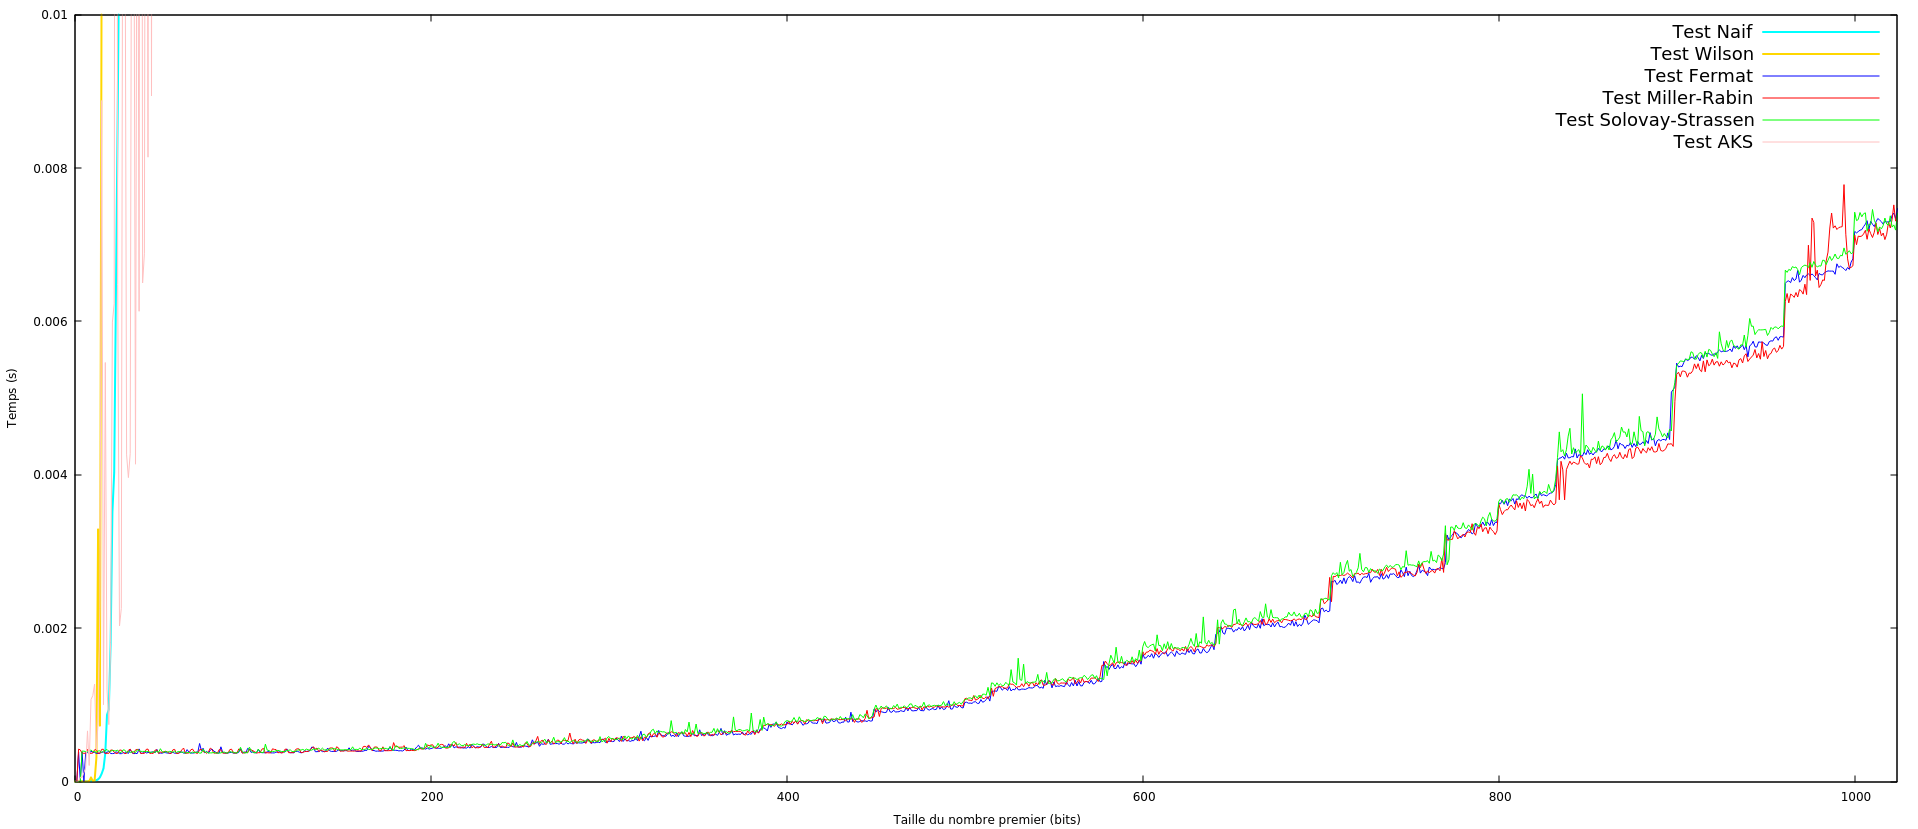
\includegraphics[width=19cm,height=11cm]{img/perfsAll.png}}\vspace{-1em}\caption{Temps d'exécution des tests en fonction de la taille en bits du nombre premier}\label{fig:M4}\end{figure}
			
			\paragraph{} Ce graphique, qui est la superposition des courbes du temps d'exécution des 6 tests de primalité implémentés, va permettre d'observer les performances des différents algorithmes de test.
			\paragraph{} On remarque tout d'abord que les 3 tests déterministes implémentés, qui sont les tests \textit{\textbf{Naif}}, \textit{\textbf{Wilson}} et \textit{\textbf{AKS}}, ont un comportement assez similaire.
			
			\begin{figure}[H]\makebox[\textwidth]{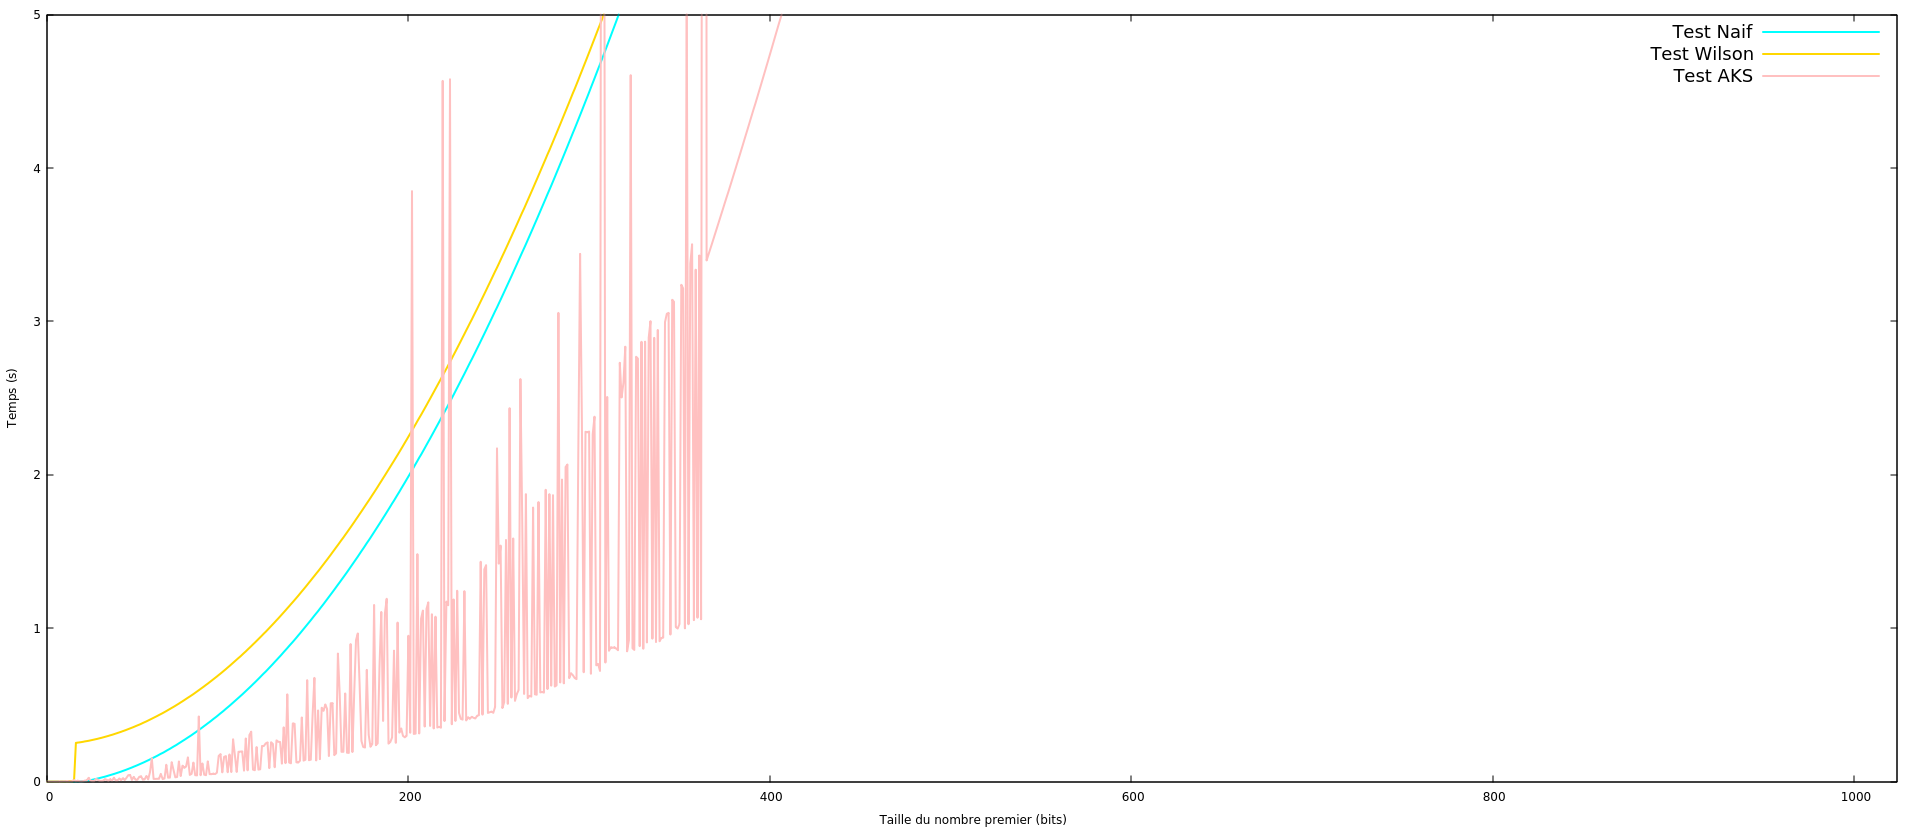
\includegraphics[width=19cm,height=11cm]{img/perfsDet.png}}\vspace{-1em}\caption{Temps d'exécution des tests déterministes}\label{fig:M5}\end{figure}
			
			\paragraph{} En effet, ces 3 tests ont un temps de réponse rapide pour un nombre de bits petit, mais ce temps de réponse va croitre d'une manière exponentielle à partir de 16 bits pour le \textit{\textbf{test Naif}} et le \textit{\textbf{test de Wilson}}, ce qui en fait des tests très lents globalement. 
			
			\paragraph{} Le \textit{\textbf{AKS}} a un temps assez variable, qui reste nettement plus rapide que le temps du \textit{\textbf{test Naif}} et du \textit{\textbf{test de Wilson}} jusqu'au nombres de taille 256 bits. Mais ce temps est relativement lent comparé aux tests probabilistes.
			
			\begin{figure}[H]\makebox[\textwidth]{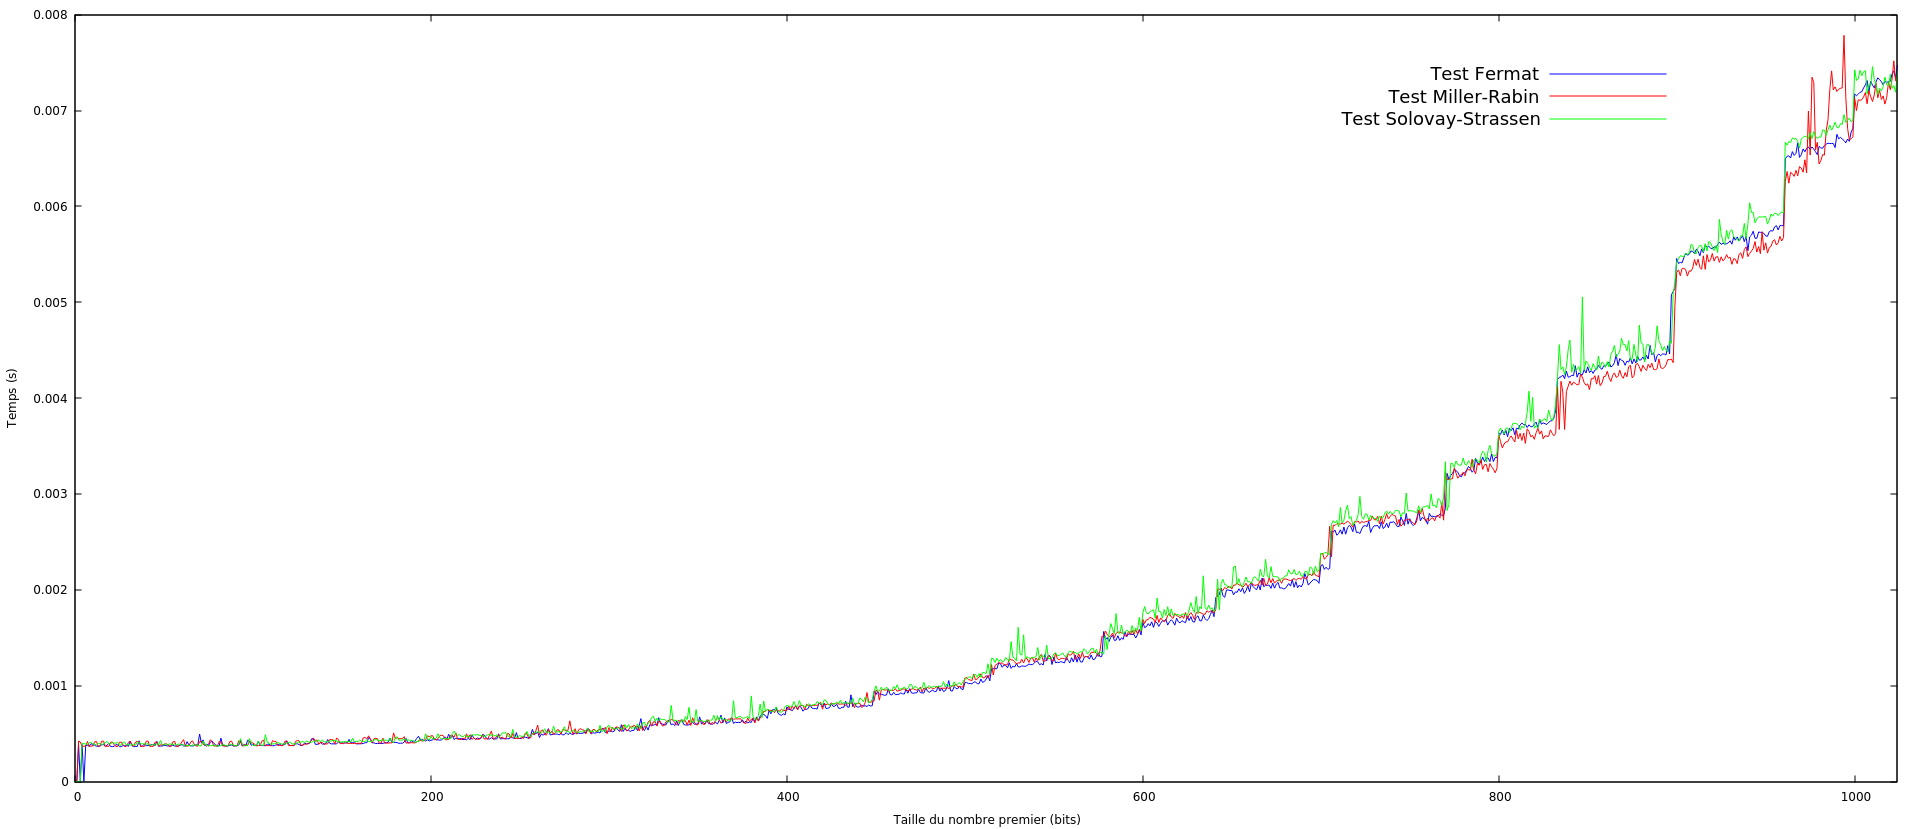
\includegraphics[width=19cm,height=11cm]{img/perfsProb.png}}\vspace{-1em}\caption{Temps d'exécution des tests probabilistes}\label{fig:M5}\end{figure}
			
			\paragraph{} Concernant les tests probabilistes, ceux-ci ont un temps d'exécution rapide en moyenne. Les 3 tests ont un temps d'exécution assez similaire avec peu de variations brusques. On remarquera surtout que le \textit{\textbf{test de Miller-Rabin}} inscrit un temps d'exécution faible en moyenne et qu'il est le plus performant quand le nombre de bits est très grand, à partir de 800 bits à peu près.

		
	\subsection{Génération optimale d'un nombre premier}
		Compte tenu des résultats des mesures effectuées sur le temps d'exécution de chaque test de primalité, il est maintenant possible, lors de la génération d'un nombre premier de $t$ bits, de choisir l'algorithme de test de primalité qui présente le temps d'exécution minimal pour $t$ bits. Pour cela, on aura juste à exploiter les résultats pré-calculés dans la structure \lstinline!tps[6][1025]! de la manière suivante :\\
			
			\begin{algorithm}[H]
				\caption{RPNG Optimal}\label{RPNG_opt}
				\Donnees{la taille $t$ en bits de l'entier premier à générer et le tableau tps[6][1025] des résultats de mesure du temps d'exécution des 6 test pour un nombre de bits entre 0 et 1024}
				\Sortie{un nombre premier de $t$ bits}
				Trouver le test de primalité d'indice $i$ ($i$ entre $0$ et $5$) telle que tps[i][t] est minimale (c'est-à-dire le test le plus rapide pour vérifier $t$ bits)\;
				Générer un nombre premier de $t$ bits avec le test de primalité d'indice $i$\;
			\end{algorithm}
			~\\
